\documentclass[10pt, sans, compress, usenames, dvipsnames, aspectratio=169]{beamer}

%% Import the template configuration
\usepackage[T1]{fontenc}
\usepackage{lmodern}
\usepackage{graphicx}
\usepackage[french]{babel}
\usepackage[utf8]{inputenc}
\usetheme{Warsaw}
\usepackage{wasysym}
\usepackage{tabularx}
\usepackage{hyperref}
\usepackage[absolute,overlay]{textpos}
\setbeamertemplate{navigation symbols}{}
\useoutertheme{infolines}
\useinnertheme{rectangles}
\setbeamertemplate{background canvas}{
\includegraphics[width=\paperwidth,height=\paperheight]{images/ucabackground-16_9.png}}
\usepackage{caption}
\captionsetup{figurename=}
\definecolor{uca01}{HTML}{006E83}
\definecolor{uca02}{HTML}{0096A0}
\definecolor{uca03}{HTML}{006C82}
\definecolor{uca04}{HTML}{0398A1}
\definecolor{uca05}{HTML}{585656}
\definecolor{uca06}{HTML}{438D97}
\definecolor{grisuca}{HTML}{5E5C5C}


\setbeamercolor{palette primary}{bg=uca06}
\setbeamercolor{palette secondary}{bg=uca03}
\setbeamercolor{palette tertiary}{bg=uca04}
\setbeamercolor{palette quaternary}{bg=uca05}
\setbeamercolor{block title}{bg=uca06}
\setbeamercolor{itemize item}{fg=uca03}
\setbeamercolor{itemize subitem}{fg=uca03}
\setbeamercolor{itemize subsubitem}{fg=uca03}


\setbeamercolor{enumerate item}{bg=uca03,fg=uca03}
\setbeamercolor{enumerate subitem}{bg=uca03,fg=uca03}
\setbeamercolor{enumerate subsubitem}{bg=uca03,fg=uca03}
\setbeamercolor{enumerate mini template}{bg=uca03,fg=uca03}
\setbeamercolor{itemize body}{fg=uca03}
\setbeamercolor{itemize subbody}{fg=uca03}
\setbeamercolor{itemize subsubbody}{fg=uca03}
\setbeamercolor{enumerate body}{fg=uca03}
\setbeamercolor{enumerate subbody}{fg=uca03}
\setbeamercolor{enumerate subsubbody}{fg=uca03}

\setbeamercolor{item projected}{bg=uca03}
\setbeamercolor{section in toc}{fg=grisuca}
\setbeamercolor{normal text}{fg=grisuca}



\title{Environment manager from your OS to your environment}
\subtitle{Encapuslation levels using docker, conda \blfootnote{This work is derived from the IFB and I2BC team members}}

\author[Pierre MARIN]{\underline{P. Marin}, M. Hiriart, P. Ruiz \& N. Goué\\\texttt{aubi@uca.fr}}
\institute{Université Clermont Auvergne, AuBi, Mésocentre}
\date{\today}
\newif\iflattersubsect

\begin{document}
\begin{frame}
  \titlepage
  \faCreativeCommons
  \begin{textblock*}{5cm}(2cm,0.5cm) % {block width} (coords)
  
\includegraphics[width=2.3cm,height=1.3cm]{logo_ifb.pdf}
  \end{textblock*}
  \begin{textblock*}{5cm}(13cm,0.3cm) % {block width} (coords)
  
\includegraphics[width=1.5cm,height=1.5cm]{i2bc.png}
  \end{textblock*}
  \begin{textblock*}{5cm}(1cm,4cm) % {block width} (coords)
  
\includegraphics[width=3.5cm,height=2.5cm]{logoAuBi-2019.pdf}
  \end{textblock*}
  \begin{textblock*}{5cm}(12cm,3.6cm) % {block width} (coords)
  
\includegraphics[width=3.5cm,height=3cm]{mesocentre.png}
  \end{textblock*}
   \begin{textblock*}{5cm}(12.8cm,6cm) % {block width} (coords)
  
\includegraphics[width=2cm,height=1cm]{medis_logo.png}
  \end{textblock*}
\end{frame}

\begin{frame}
  \frametitle{Contents}
  \begin{multicols*}{2}
  \tableofcontents
  \end{multicols*}
\end{frame}

\section{A common use-case}
\subsection{Retry my results}

\begin{frame}{A classic use case}
\centering{
\onslide<1->{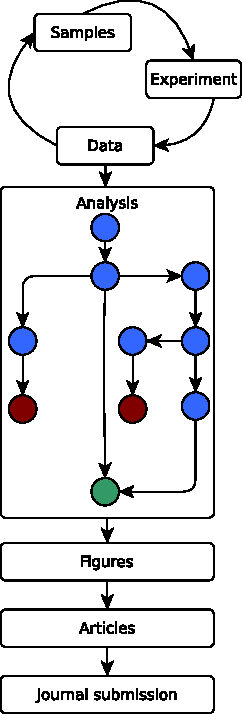
\includegraphics[width=0.17\textwidth]{schema_soumission_fair.pdf}}
\onslide<2->{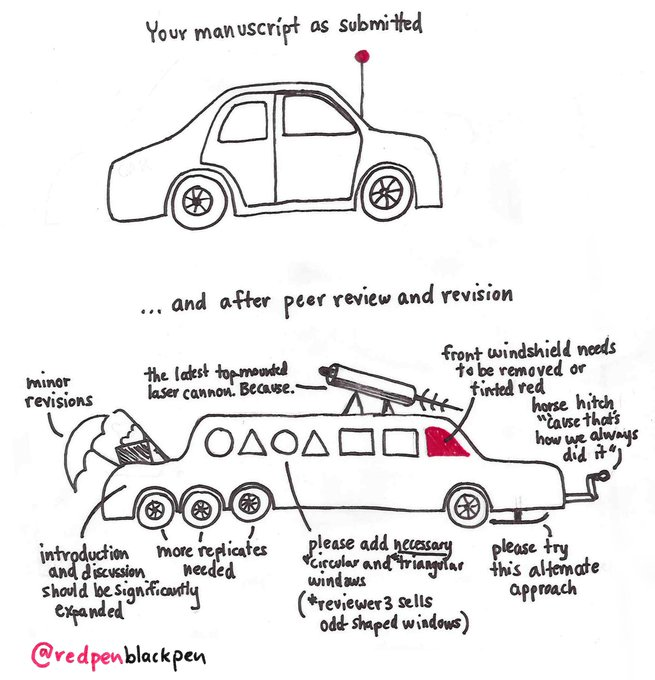
\includegraphics[width=0.4\textwidth]{review.jpg}}
\onslide<3->{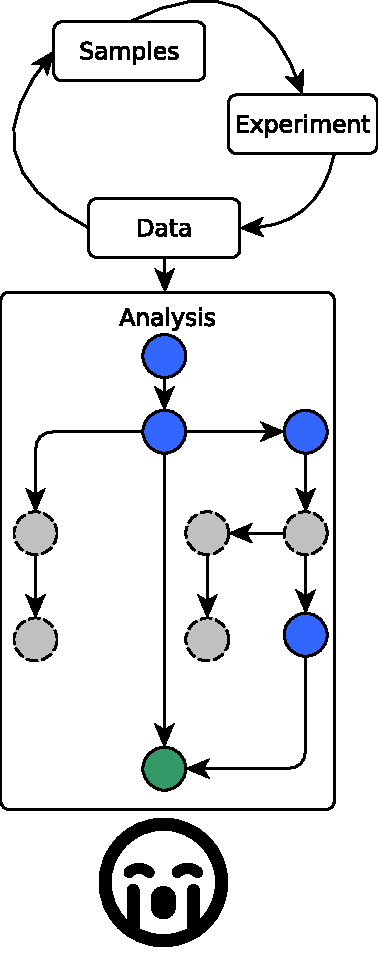
\includegraphics[width=0.17\textwidth]{schema_soumission_fair_echec.pdf}}}
\end{frame}
\begin{frame}{A classic use case}
\centering{What are the changes ?}
\begin{columns}
\column{.5\textwidth}
\begin{itemize}
	\item Tool version
	\item Packages
	\item Environment variables
\end{itemize}
\column{.5\textwidth}
\begin{itemize}
	\item OS version
	\item The computer 
	\item ...
\end{itemize}
\end{columns}
\end{frame}

\begin{frame}
\begin{itemize}
\item Tool compatibility troubles
	\begin{itemize}
	\item Python version ? 2.7, 3.8...
	\item Which tool version ?
	\item Installation without root access
	\item coexistance bewteen severals versions, libraries
	\end{itemize}
\end{itemize}
\end{frame}

\begin{frame}{My python env}
\centering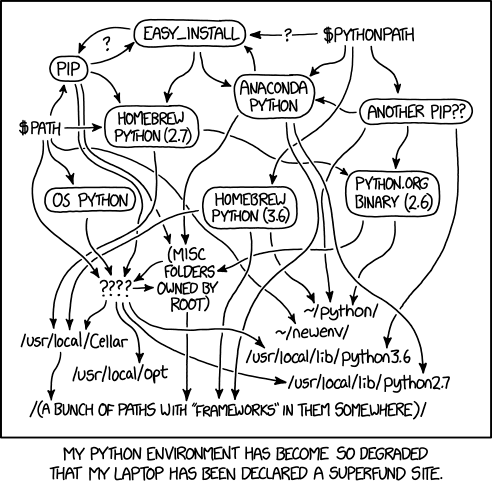
\includegraphics[width=0.5\textwidth]{python_environment.png} 
\end{frame}

\subsection{The use of packaging}
\begin{frame}[<+->]{Encapsulation levels}
\textit{Encapsulation: capture the environment of applications (OS, packages, libraries) to control their execution}
\begin{itemize}[<+->]
	\item Environment management (package manager) 
\includegraphics[width=0.09\textwidth]{conda_logo.pdf} 
	\item Hardware virtualisation (virtual machines) 
\includegraphics[width=0.09\textwidth]{VM_logo.png} 
	\item OS virtualisation (images and containers) 
\includegraphics[width=0.09\textwidth]{docker.pdf} 
\includegraphics[width=0.09\textwidth]{singularity_logo.pdf} 

\end{itemize}
\end{frame}

\subsection{Example with R}
\begin{frame}{Example of R and package installation}{Classical installation}
\begin{itemize}[<+->]
	\item Start with a computer and a specific OS
	\item Inside, we installed a new 
\includegraphics[width=0.3cm, height=0.3cm]{r-project.pdf} application
	\item 
\includegraphics[width=0.3cm, height=0.3cm]{r-project.pdf} need some dependencies
	\item We tested the last  
\includegraphics[width=0.3cm, height=0.3cm]{r-project.pdf} version --> might be conflicts
\end{itemize}

\onslide<1->{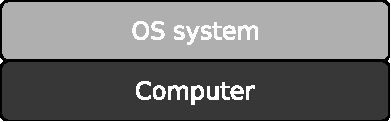
\includegraphics[width=0.25\textwidth]{conda_env_1.pdf}}
\onslide<2->{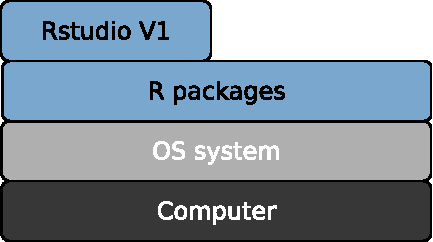
\includegraphics[width=0.25\textwidth]{conda_env_2.pdf}}
\only<3>{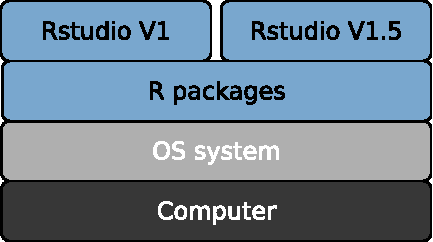
\includegraphics[width=0.25\textwidth]{conda_env_3.pdf}}
\onslide<4->{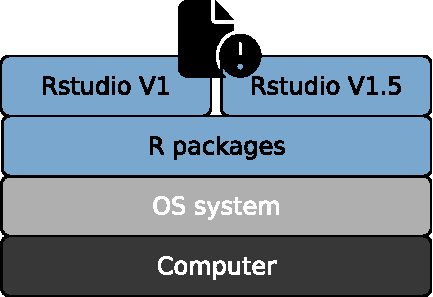
\includegraphics[width=0.25\textwidth]{conda_env_4.pdf}}
\end{frame}


\section{Manage your local environment}
\subsection{How conda works}
\begin{frame}[<+->]{Example of R and package installation}{Conda use}
\begin{itemize}
	\item The idea is to separate each application in here own environment 
\includegraphics[width=0.1\textwidth]{images/conda_logo.pdf}
	\item A tool version, a conda environment
	\item Create a new environment for my new tool version, my analysis...
\end{itemize}
\onslide<1->{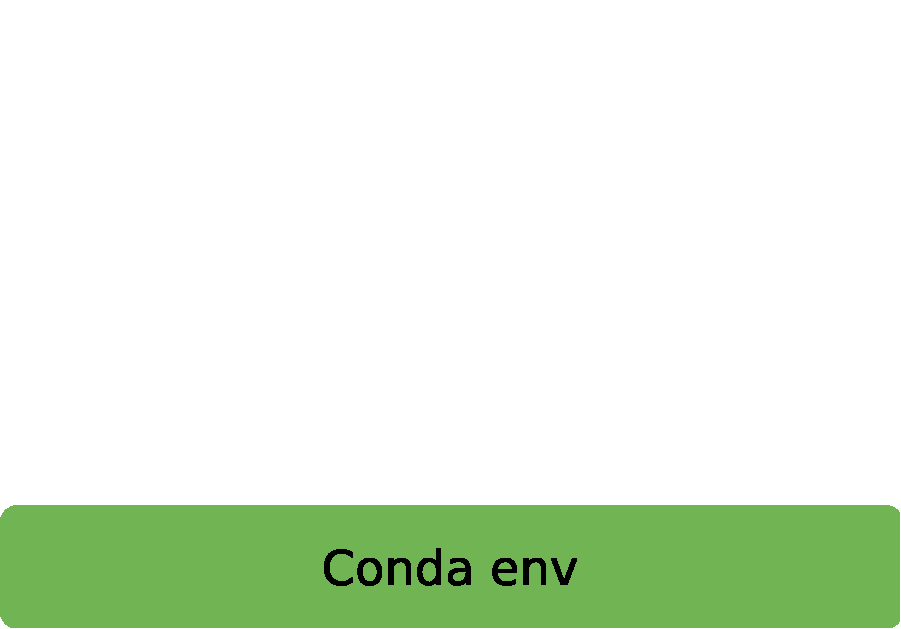
\includegraphics[width=0.3\textwidth]{images/conda_env_5.pdf}}
\onslide<2->{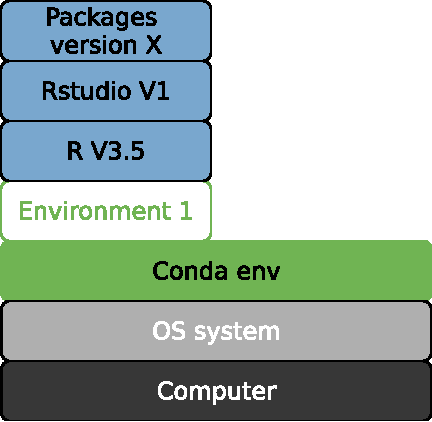
\includegraphics[width=0.3\textwidth]{images/conda_env_6.pdf}}
\onslide<3->{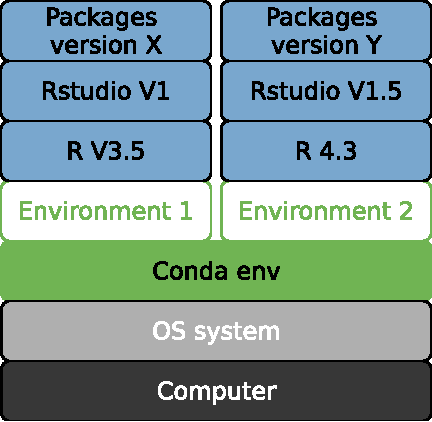
\includegraphics[width=0.3\textwidth]{images/conda_env_7.pdf}}
\end{frame}

\section{Manage your hardware configuration}
\subsection{How virtual manager works}

\begin{frame}{Example of R and package installation}{hardware virtualisation}
\begin{columns}
\column{.5\textwidth}
\begin{itemize}[<+->]
	\item If we want a software from a different OS ?
	\item Use virtual machines
	\item Each application get a total different and independant environment
	\item Virtual machine could be transfered to another computer
\end{itemize}
\column{.5\textwidth}
\begin{itemize}[<+->]
	\item Redundancy between VMs
	\item Heavy to set up
	\item No automation
\end{itemize}
\end{columns}
\onslide<1-3>{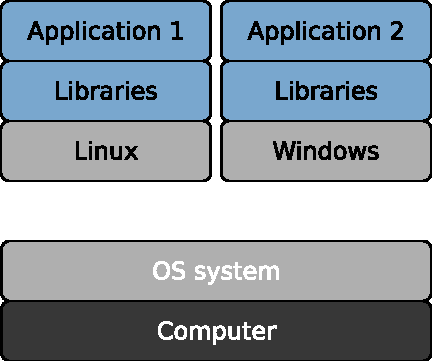
\includegraphics[width=0.3\textwidth]{images/VM_env_1.pdf}}
\onslide<2-3>{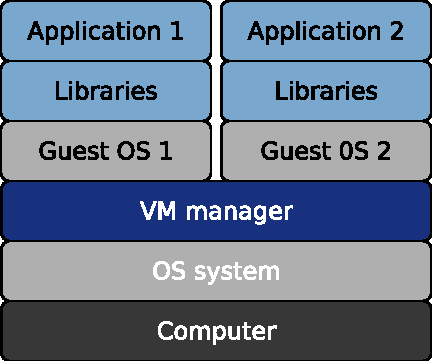
\includegraphics[width=0.3\textwidth]{images/VM_env_2.pdf}}
\begin{textblock*}{10cm}(2cm,4.5cm) % {block width} (coords)
\onslide<4->{\centering{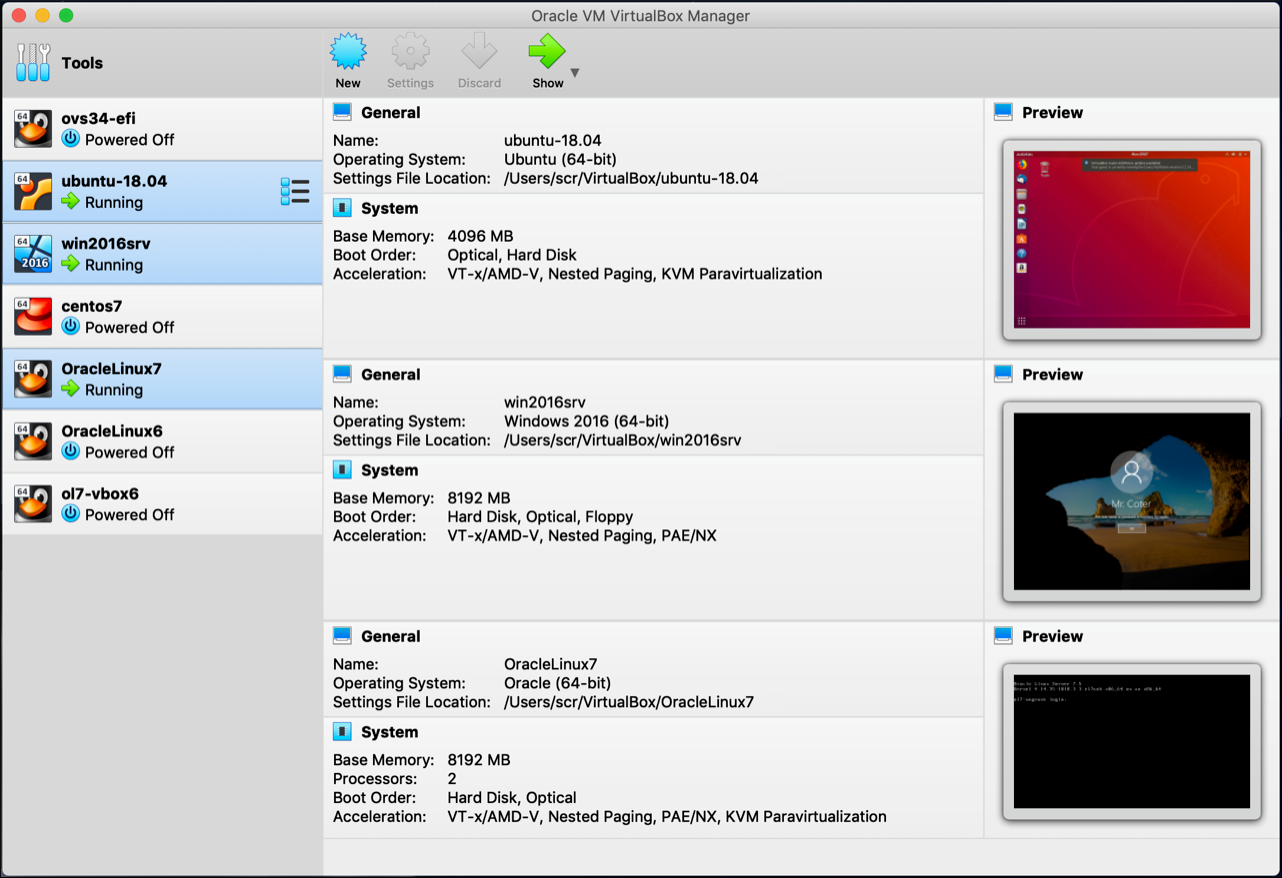
\includegraphics[width=0.6\textwidth]{images/virtualbox-main.png}}}
\end{textblock*}
\end{frame}


\section{Manage your OS configuration}
\subsection{How container works}

\begin{frame}{Example of R and package installation}{OS virtualisation}
\begin{columns}
\column{.5\textwidth}
\begin{itemize}[<+->]
	\item "Trick" applications into believing that they are in a different OS than the host’s
	\item Named containers: 
\includegraphics[width=2cm, height=0.5cm]{images/docker_logo2.png} or 
\includegraphics[width=0.8cm, height=0.8cm]{images/singularity_logo.pdf}
	\item Avoid redundancy
	\item<5-> Speed
	\begin{itemize}[<5->]
		\item Faster installation
		\item No boot time
	\end{itemize}
	\item<6-> Lightweight
	\begin{itemize}[<6->]
		\item Minimal base OS
		\item Minimal set of library and global environment 
		\item Easy sharing of application 
	\end{itemize}	
\end{itemize}
\column{.5\textwidth}
\begin{itemize}[<8->]
	\item No easy use on a cluster system
	\item Docker private company policies
\end{itemize}
\end{columns}

\begin{textblock*}{10cm}(1cm,7.2cm) % {block width} (coords)
\onslide<3-4>{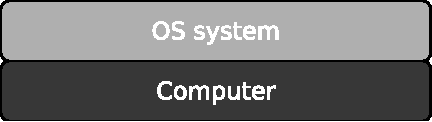
\includegraphics[width=4cm, height=1cm]{images/docker_env_1.pdf}}
\end{textblock*}
\begin{textblock*}{10cm}(6cm,4.5cm) % {block width} (coords)
\onslide<4-4>{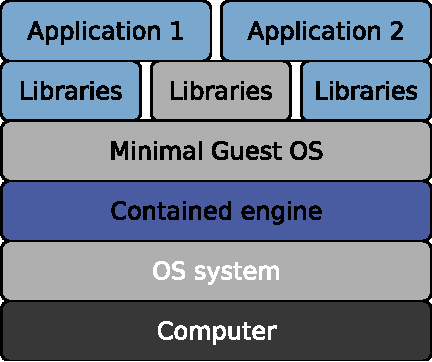
\includegraphics[width=4cm, height=3.7cm]{images/docker_env_2.pdf}} 
\end{textblock*}
\begin{textblock*}{10cm}(8cm,3cm) % {block width} (coords)
\onslide<6-6>{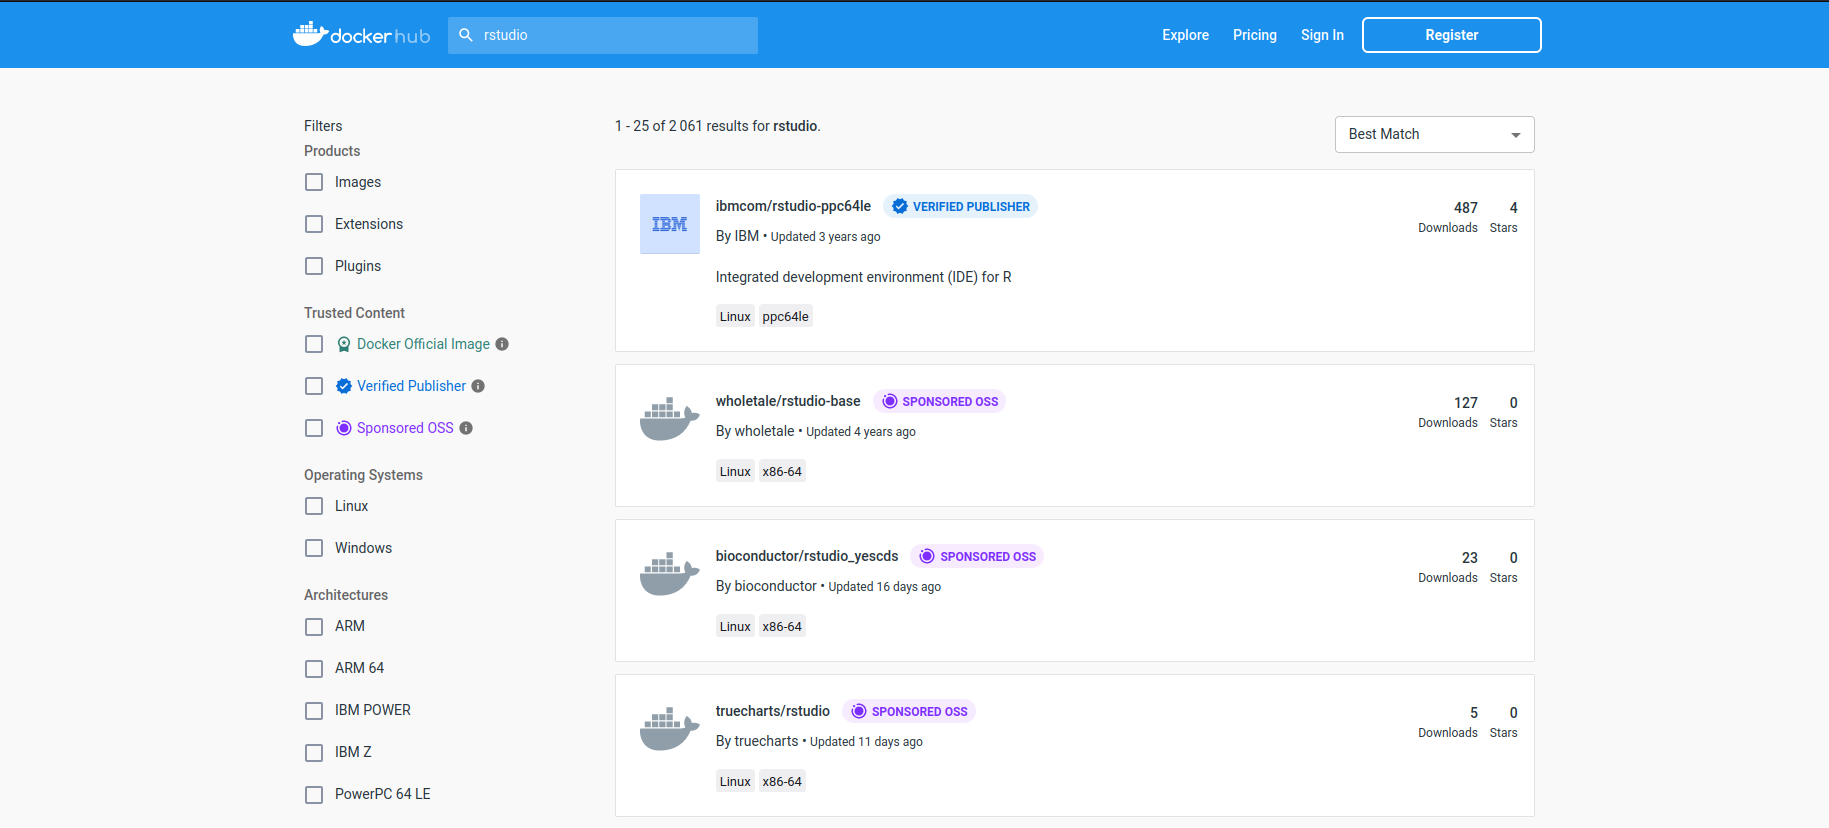
\includegraphics[width=0.9\textwidth]{images/docker_hub.png}}
\end{textblock*}
\begin{textblock*}{10cm}(8cm,3cm) % {block width} (coords)
\onslide<7-7>{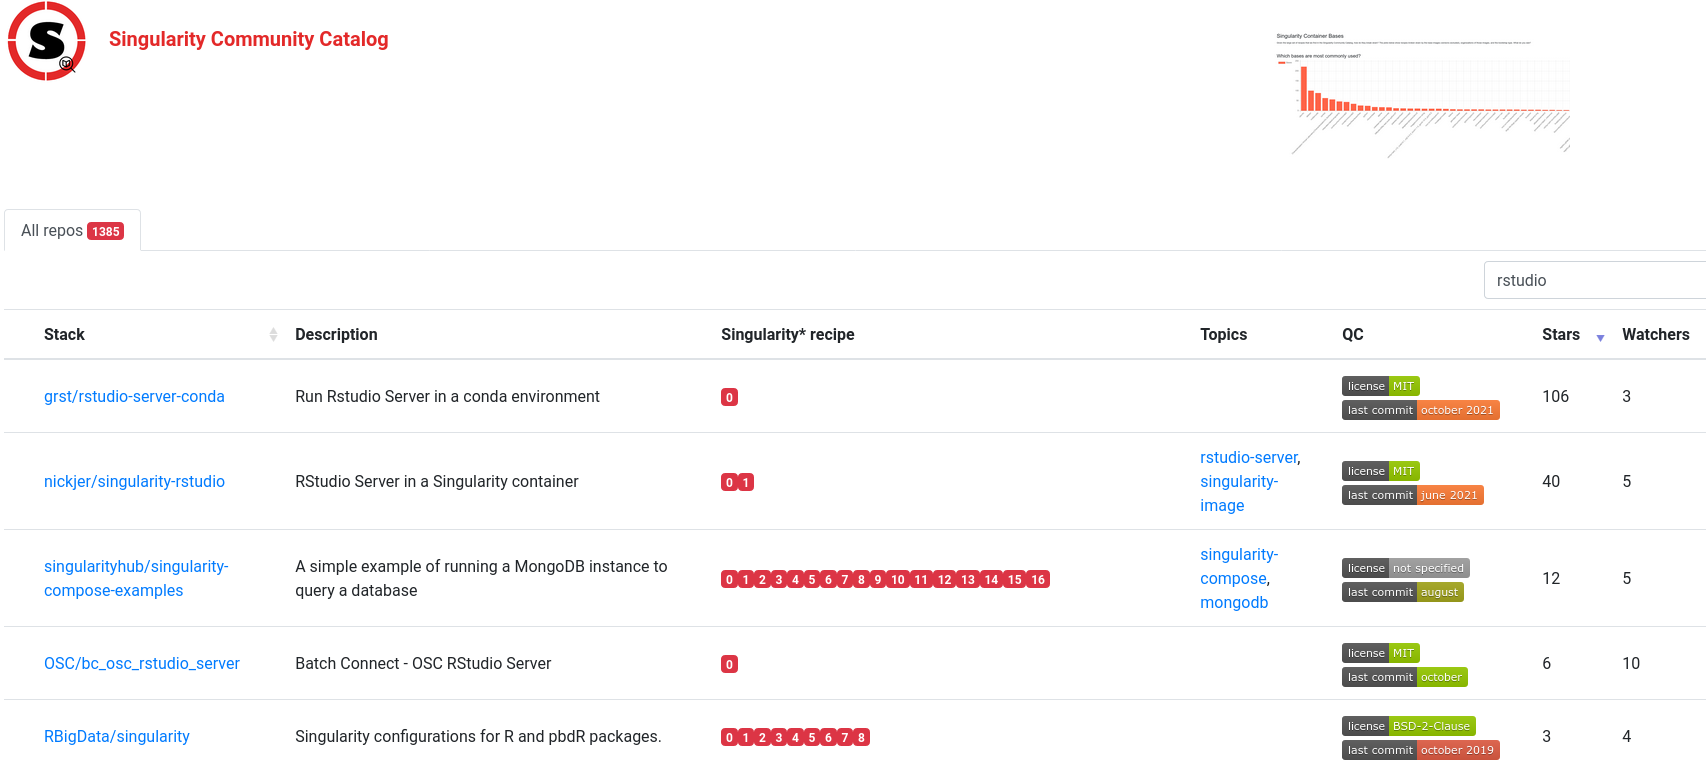
\includegraphics[width=0.9\textwidth]{images/singularity_hub.png}}
\end{textblock*}
\begin{textblock*}{10cm}(0.4cm,1cm) % {block width} (coords)
\onslide<8->{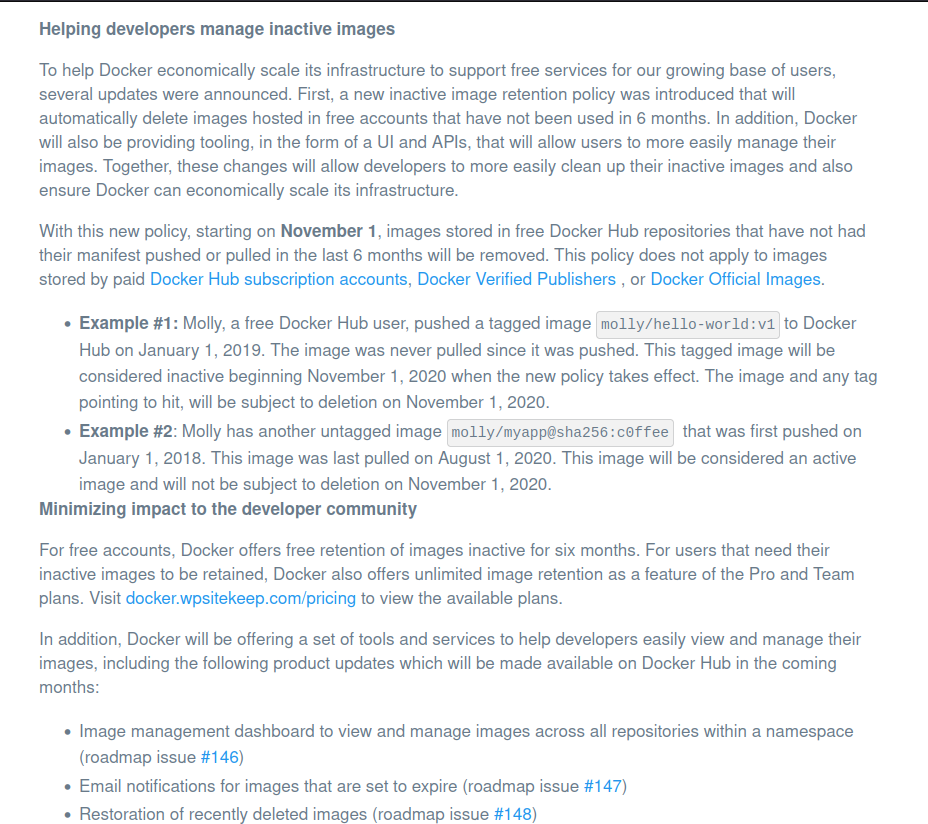
\includegraphics[width=0.8\textwidth]{images/docker_retention.png}}\onslide<8->{\footnote{\url{https://www.docker.com/blog/scaling-docker-to-serve-millions-more-developers-network-egress/}}}
\end{textblock*}

\end{frame}
\section{Conda ecosystem}
\subsection{a case of bioconda}

\begin{frame}{Conda system}
\begin{itemize}
\item<2-4> \hyperlink{https://www.anaconda.com/}{Anaconda}
	\begin{itemize}
	\item Open source distribution
    \item Cross platform
    \item Available on cluster without admin whrite
    \item Thousands of available tool in informatic and bioinformatic
	\end{itemize}
\item<3-4> \hyperlink{https://docs.conda.io/en/latest/miniconda.html}{Miniconda}
	\begin{itemize}
	\item A lightheight Anaconda version with minimal requirment
	\item Same advantages ad Anaconda
	\end{itemize}
\item<4-4> \hyperlink{https://docs.conda.io/projects/conda/en/latest/index.html}{Conda} 
\includegraphics[width=0.1\textwidth]{images/conda_logo.pdf} 
	\begin{itemize}[<4->]
	\item Package manager AND environment manager
	\item installed with Ana or Miniconda
	\item Python based but can also install tools from R, C++ or Julia...
	\end{itemize}
\end{itemize}
\end{frame}

\begin{frame}{Conda system}
\centering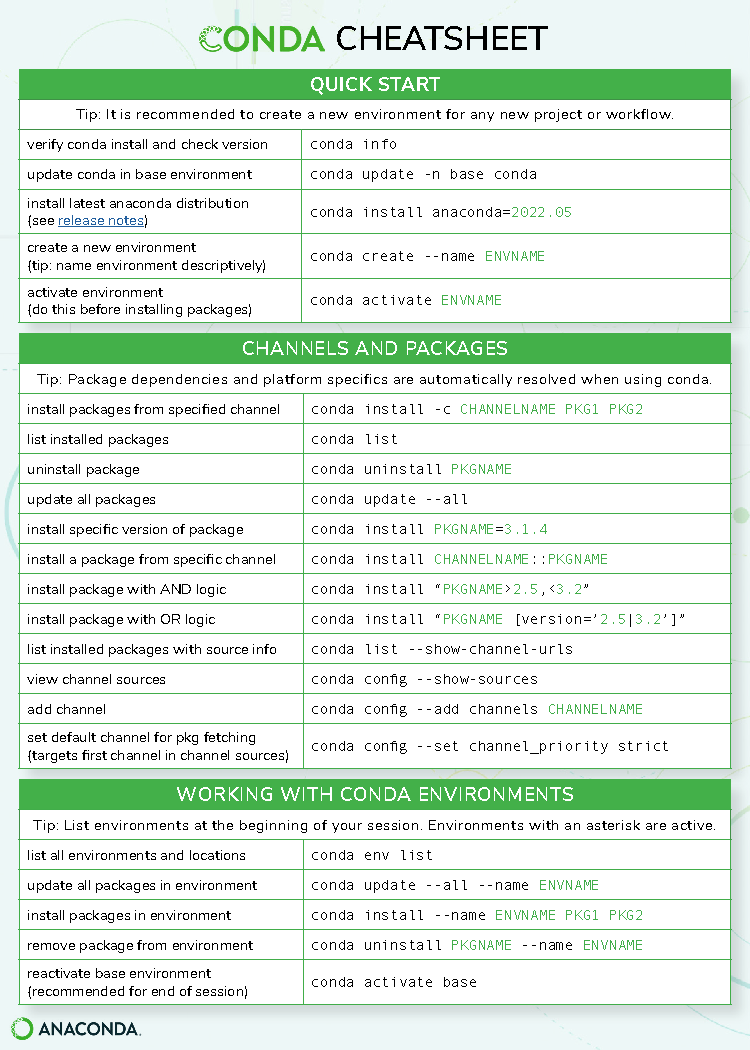
\includegraphics[width=0.45\textwidth]{images/conda_sheet_4.12.pdf}
\end{frame}
\begin{frame}{The channels and the tools}
The tools are packaged and available on several \textbf{channels}
\begin{minipage}[t]{0.48\linewidth}
\begin{itemize}[<2->]
\item Conda-forge
\item Anaconda
\end{itemize}
\end{minipage}
\begin{minipage}[t]{0.48\linewidth}
\begin{itemize}[<2->]
\item R
\item Bioconda --> Most of the bioinformatic tools
\end{itemize}
\end{minipage}
\onslide<3->{\centering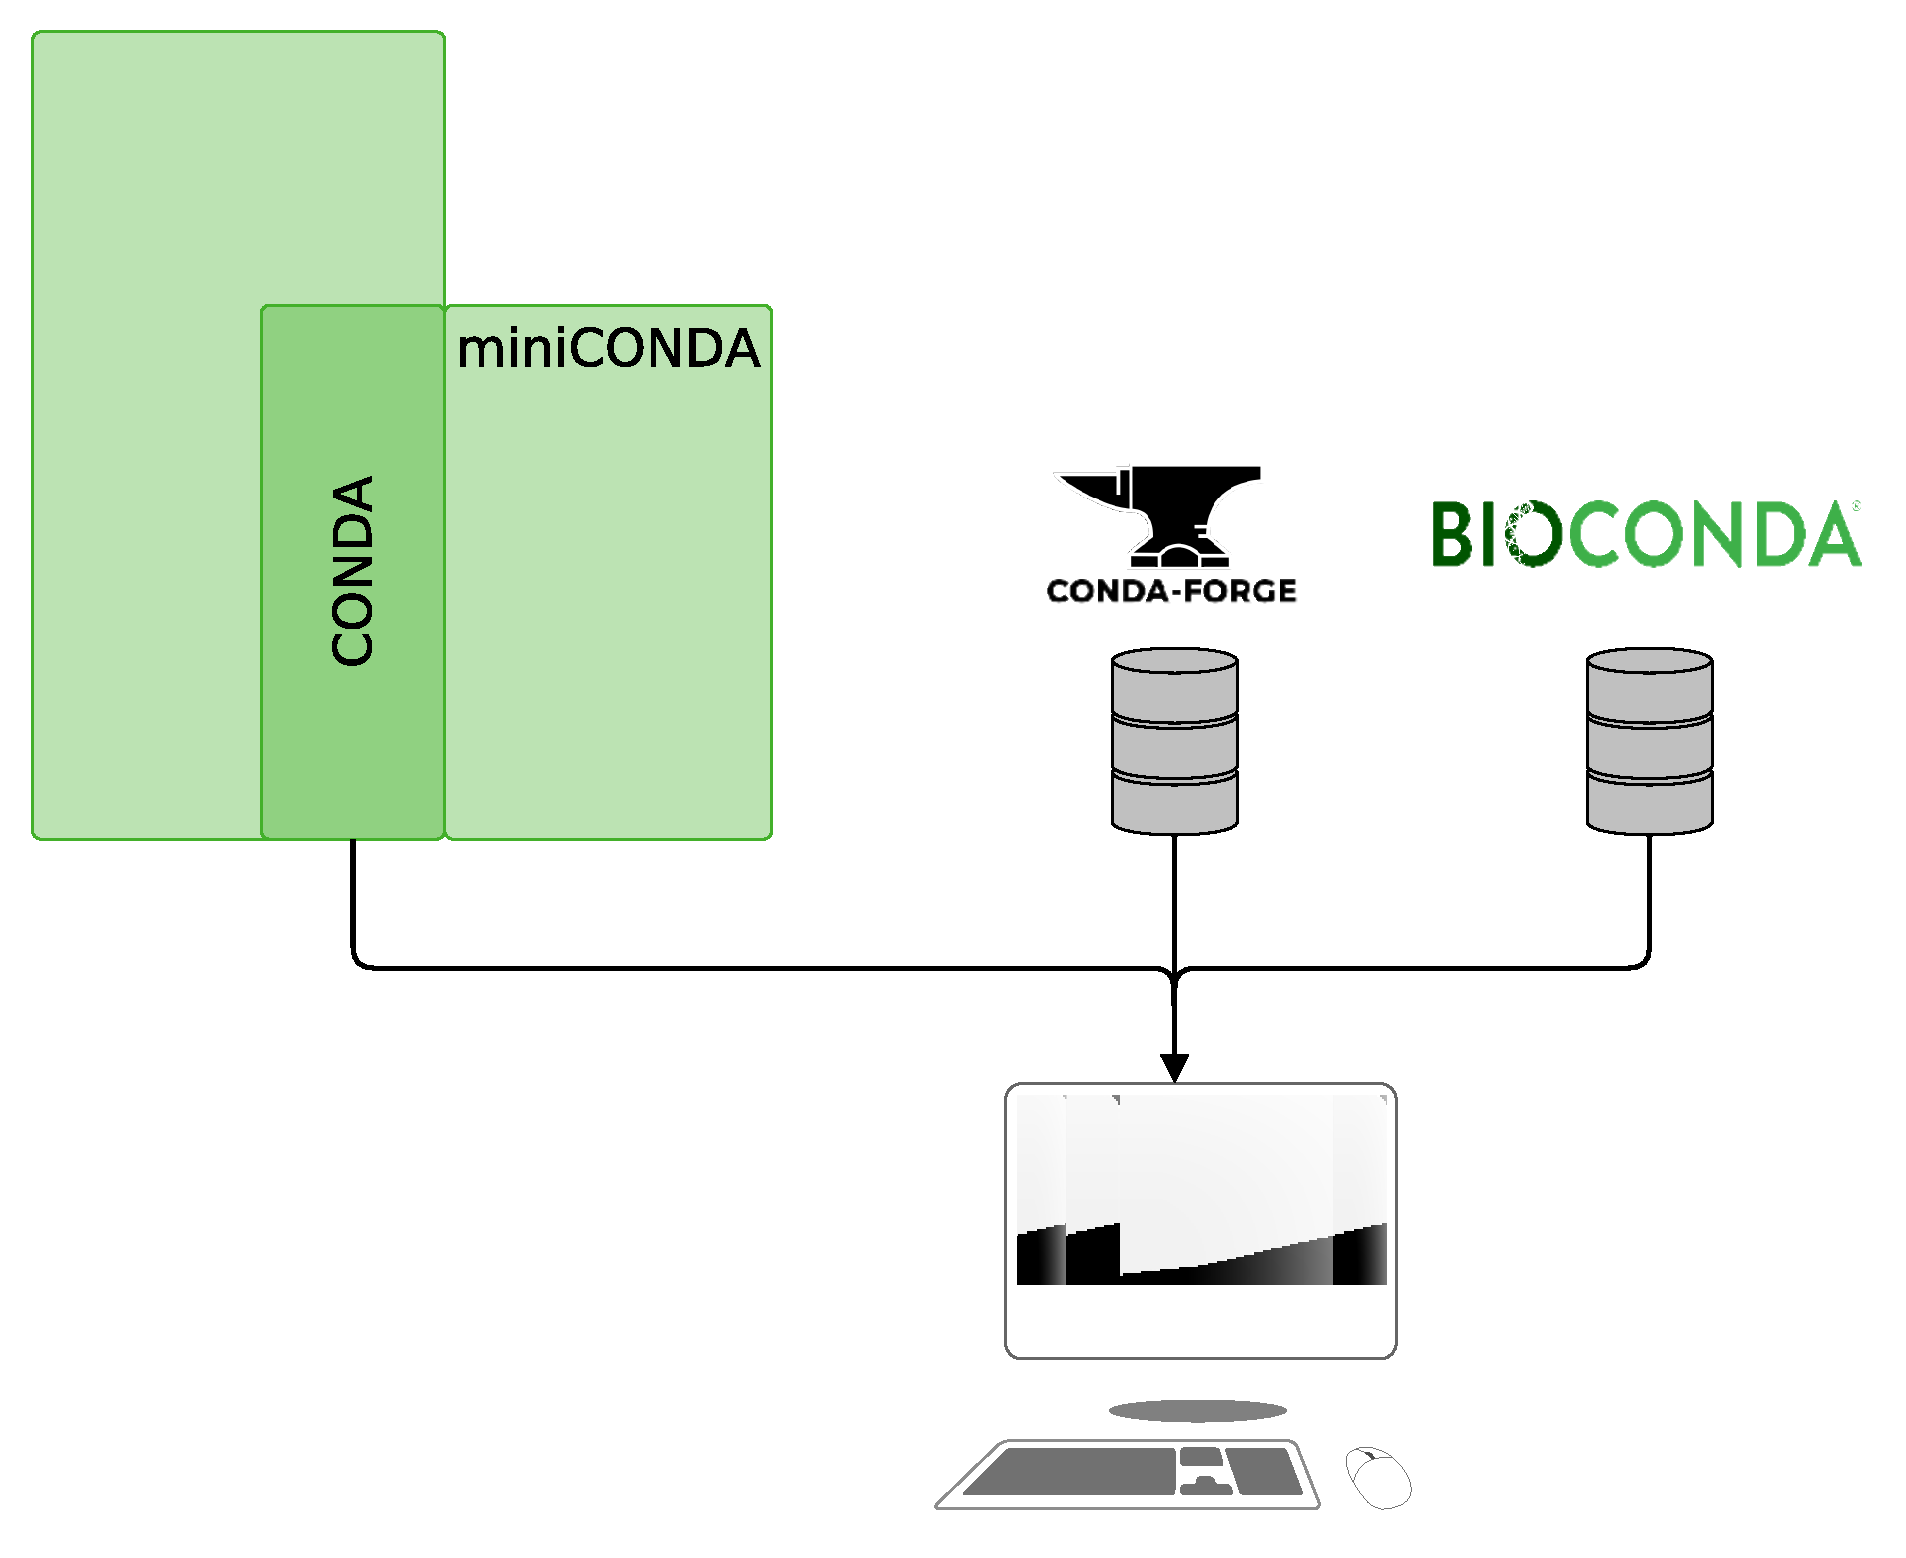
\includegraphics[width=0.5\textwidth]{images/conda_env_detail.pdf}\blfootnote{Bioconda: sustainable and comprehensive software distribution for the life sciences \textit{Grüning et al.}, Nature methods, 2018. DOI 10.1038/s41592-018-0046-7}}
\end{frame}

\begin{frame}{Basic commands}
\begin{columns}
\column{.48\textwidth}
\onslide<1->{
\begin{block}{Create environment}
\begin{itemize}
\item[\$] conda create -n [env\_name]
\item[\$] conda activate [env\_name]
\item[\$] conda deactivate [env\_name]
\end{itemize}
\end{block}}
\onslide<2->{
\begin{block}{list environment or packages}
\begin{itemize}
\item[\$] conda env list
\item[\$] conda list
\end{itemize}
\end{block}}
\column{.48\textwidth}
\onslide<3->{
\begin{block}{Search tools}
\begin{itemize}
\item[\$] conda search bowtie2
\item[\$] conda search -c bioconda bowtie2
\end{itemize}
\end{block}}
\onslide<4->{
\begin{block}{Install tools}
\begin{itemize}
\item[\$] conda install bowtie2
\item[\$] conda install -c bioconda bowtie2
\item[\$] conda install -c bioconda bowtie2=2.4.5
\end{itemize}
\end{block}}
\onslide<5->{
\begin{block}{Remove tools}
\begin{itemize}
\item[\$] conda remove bowtie2
\end{itemize}
\end{block}}
\end{columns}
\end{frame}
\begin{frame}{Environment resolution}
Conda also manage your environment to install compatible tools in the same environment
\begin{itemize}[<2->]
\item time to solve the environement installation plan
\item could be locked and don't install a tool
\end{itemize}
\onslide<3->{\centering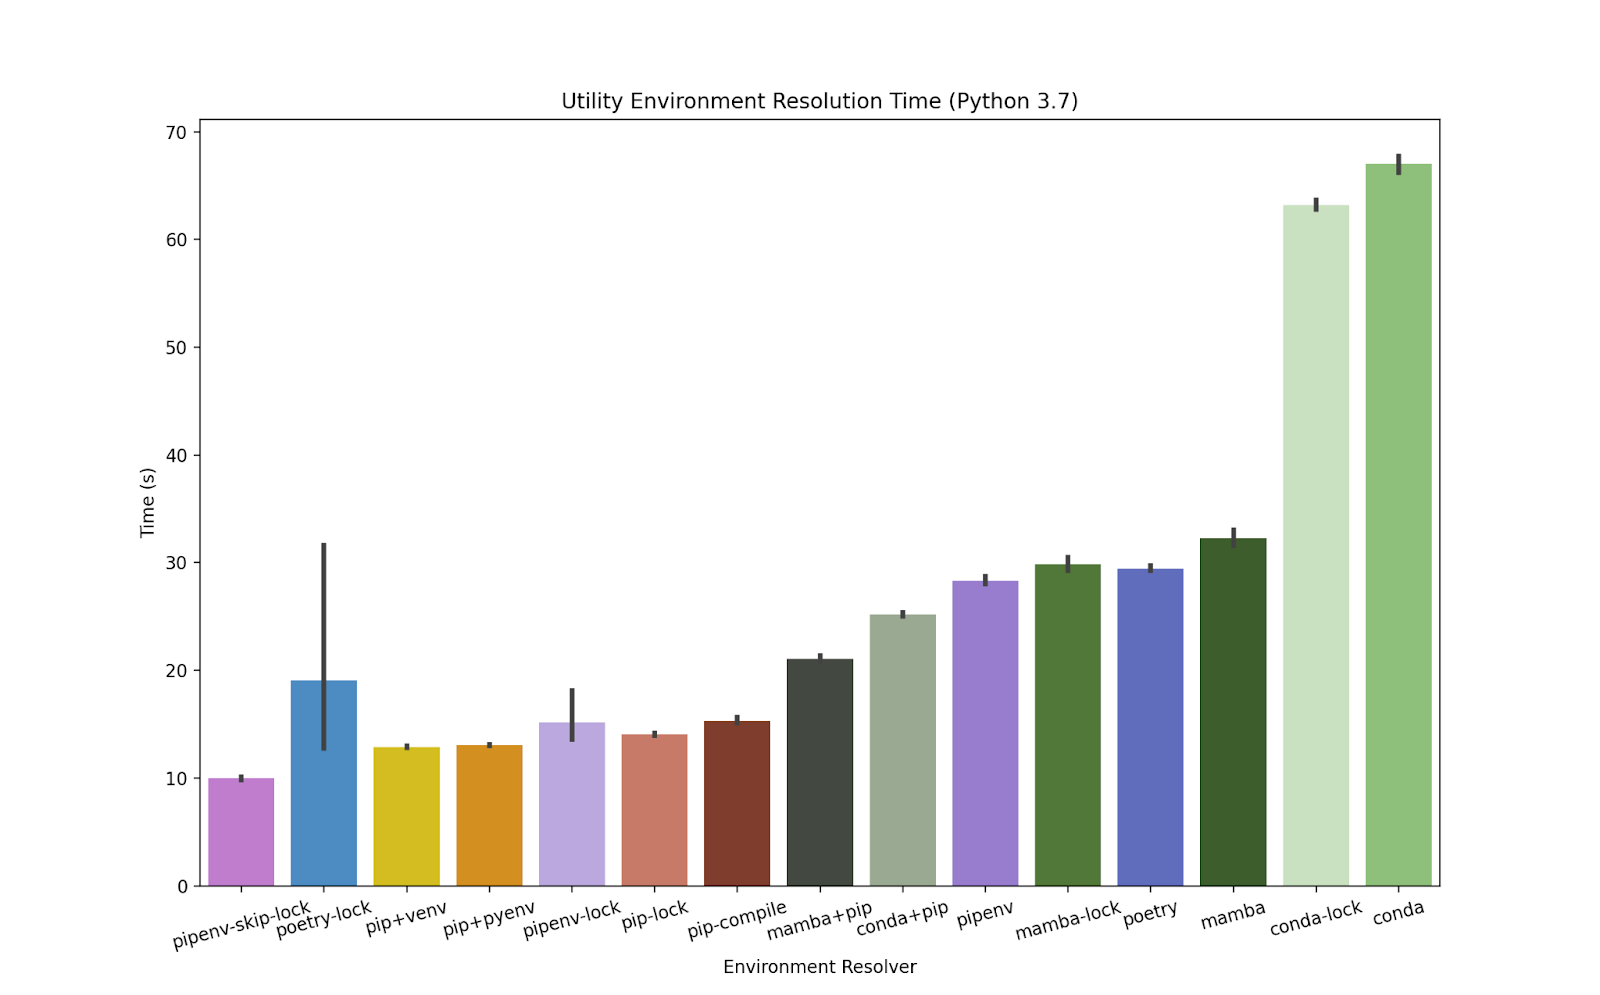
\includegraphics[width=0.7\textwidth]{images/conda_use.png}}
\end{frame}


d
\begin{frame}
\centering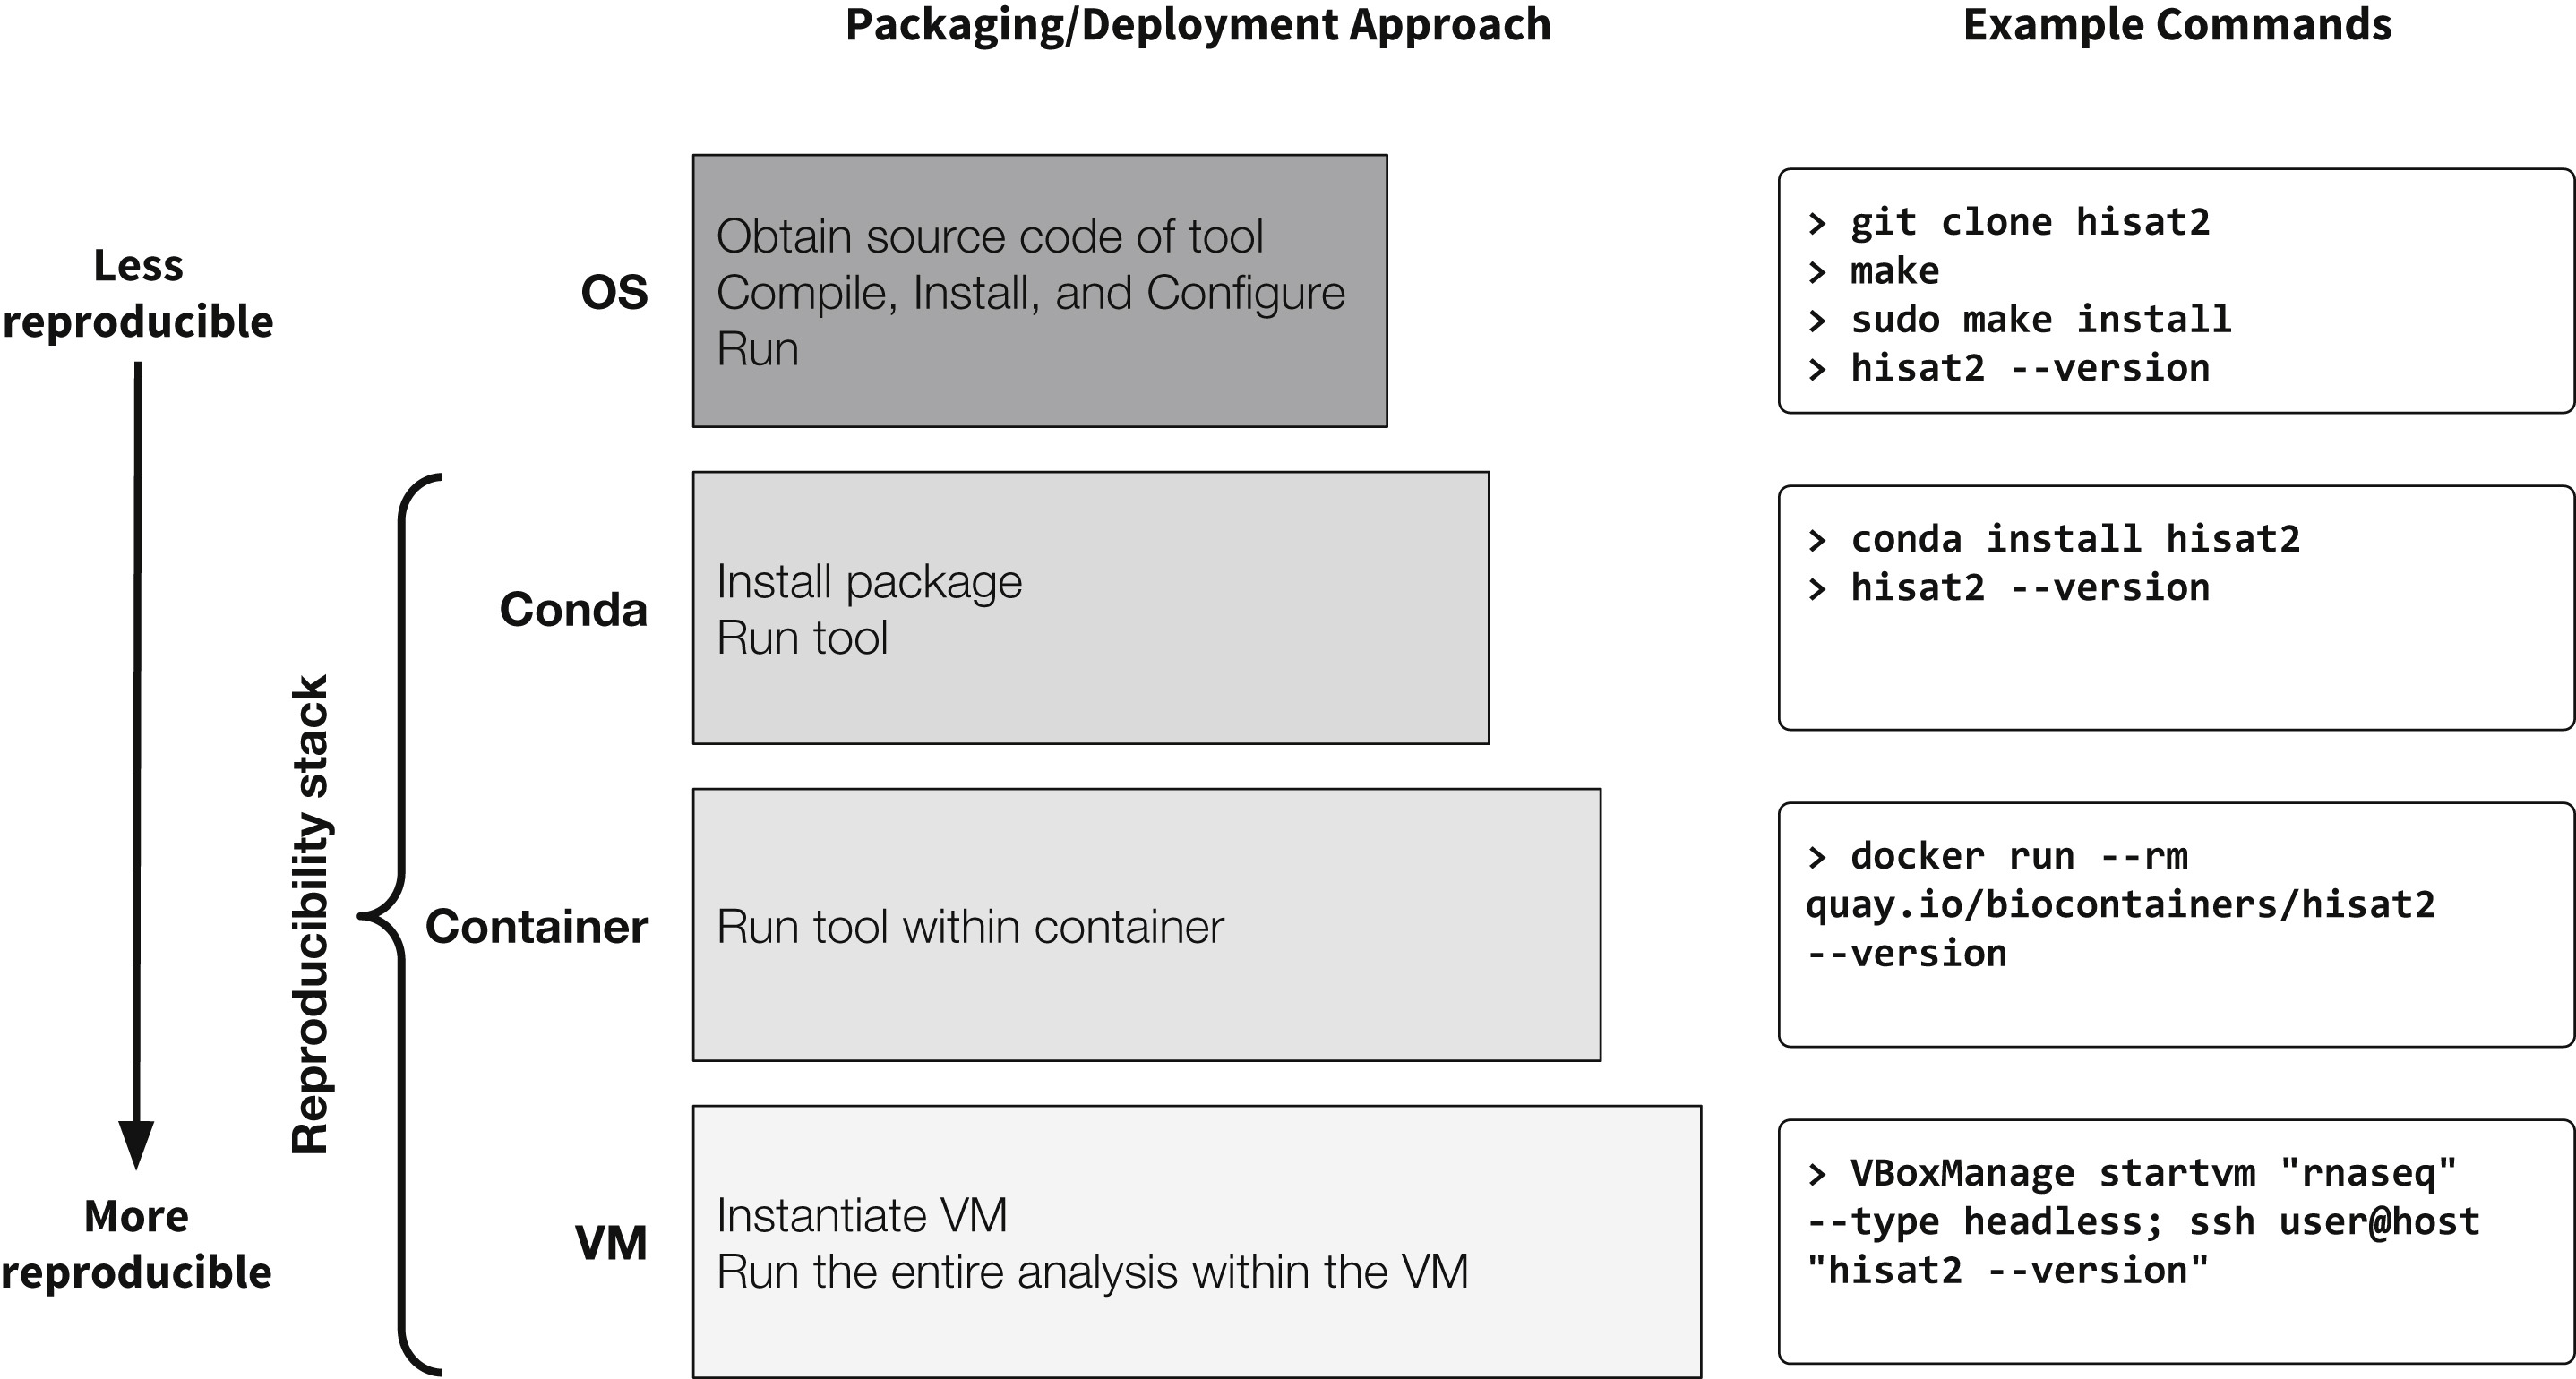
\includegraphics[width=0.8\textwidth]{images/reproductibility.jpg} \footnote{Practical Computational Reproducibility in the Life Sciences
Grüning et al, Cell Systems, 2018. DOI 10.1016/j.cels.2018.03.014}
\end{frame}
%% A METTRE EN FIN DE DIAPO
\begin{frame}[<+->]
Some recommandations \footnote{Recommendations for the packaging and containerizing of bioinformatics software Gruening, F1000 Research, 2019. DOI 10.12688/f1000research.15140.2}
\begin{itemize}
\item A package first
\item One tool, one container
\item Tool and container versions should be explicit
\item Avoid using ENTRYPOINT
\item Reduce the size of your container as much as possible
\item Keep data outside of the container
\item Add functional testing logic
\item Check the license of the software
\item Make your package or container discoverable
\item Provide reproducible and documented builds
\item Provide helpful usage message
\end{itemize}
\end{frame}
\end{document}

